\section{Qualität der Weltkarte \dcfirstauthorshort}
\label{ssec:evaluation:messungen:weltkarte}
Alle für die Regelung notwendigen Informationen über den Verlauf der Straßenmarkierungen stammen aus der parallel angelegten Karte. Damit eine stabile Navigation möglich ist, muss ihre Reliabilität vorausgesetzt sein. Die Authentizität der Kartenpunkte hängt wiederum von der Zuverlässigkeit der Pose ab. Da IMU und Encoder fehlerbehaftet sind, ist eine Abweichung der ermittelten zur realen Pose zu erwarten. 

Um die tatsächliche Genauigkeit der Pose und Weltkarte anschaulich darzustellen, wurden in Abbildung~\ref{fig:evaluation:riverflow:weltkarte:qualitaet} die geplotteten Karten- und Posendaten maßstabsgerecht über die Entwurfszeichnung gelegt. Trotz sich theoretisch aufsummierender Fehler ist die Abweichung der End- zur Startpose nach einer Runde erstaunlich gering.

\begin{figure}[htbp] % [htb]
	\centering
	
	\subfloat[Kombination des Plots der durch Messungen entstandenen Weltkarte mit der realen Entwurfszeichnung in passender Größe als Qualitätsnachweis 
	\label{fig:evaluation:riverflow:weltkarte:qualitaet}]{\includegraphics[height=0.31\textheight]{strassenszenario_kombi_weltkarte.pdf}}
	\hfill
	\subfloat[Plot der durch Messungen entstandenen Weltkarte nach einer gefahrenen Runde im Uhrzeigersinn
	\label{fig:evaluation:riverflow:weltkarte:andere_Richtung}]{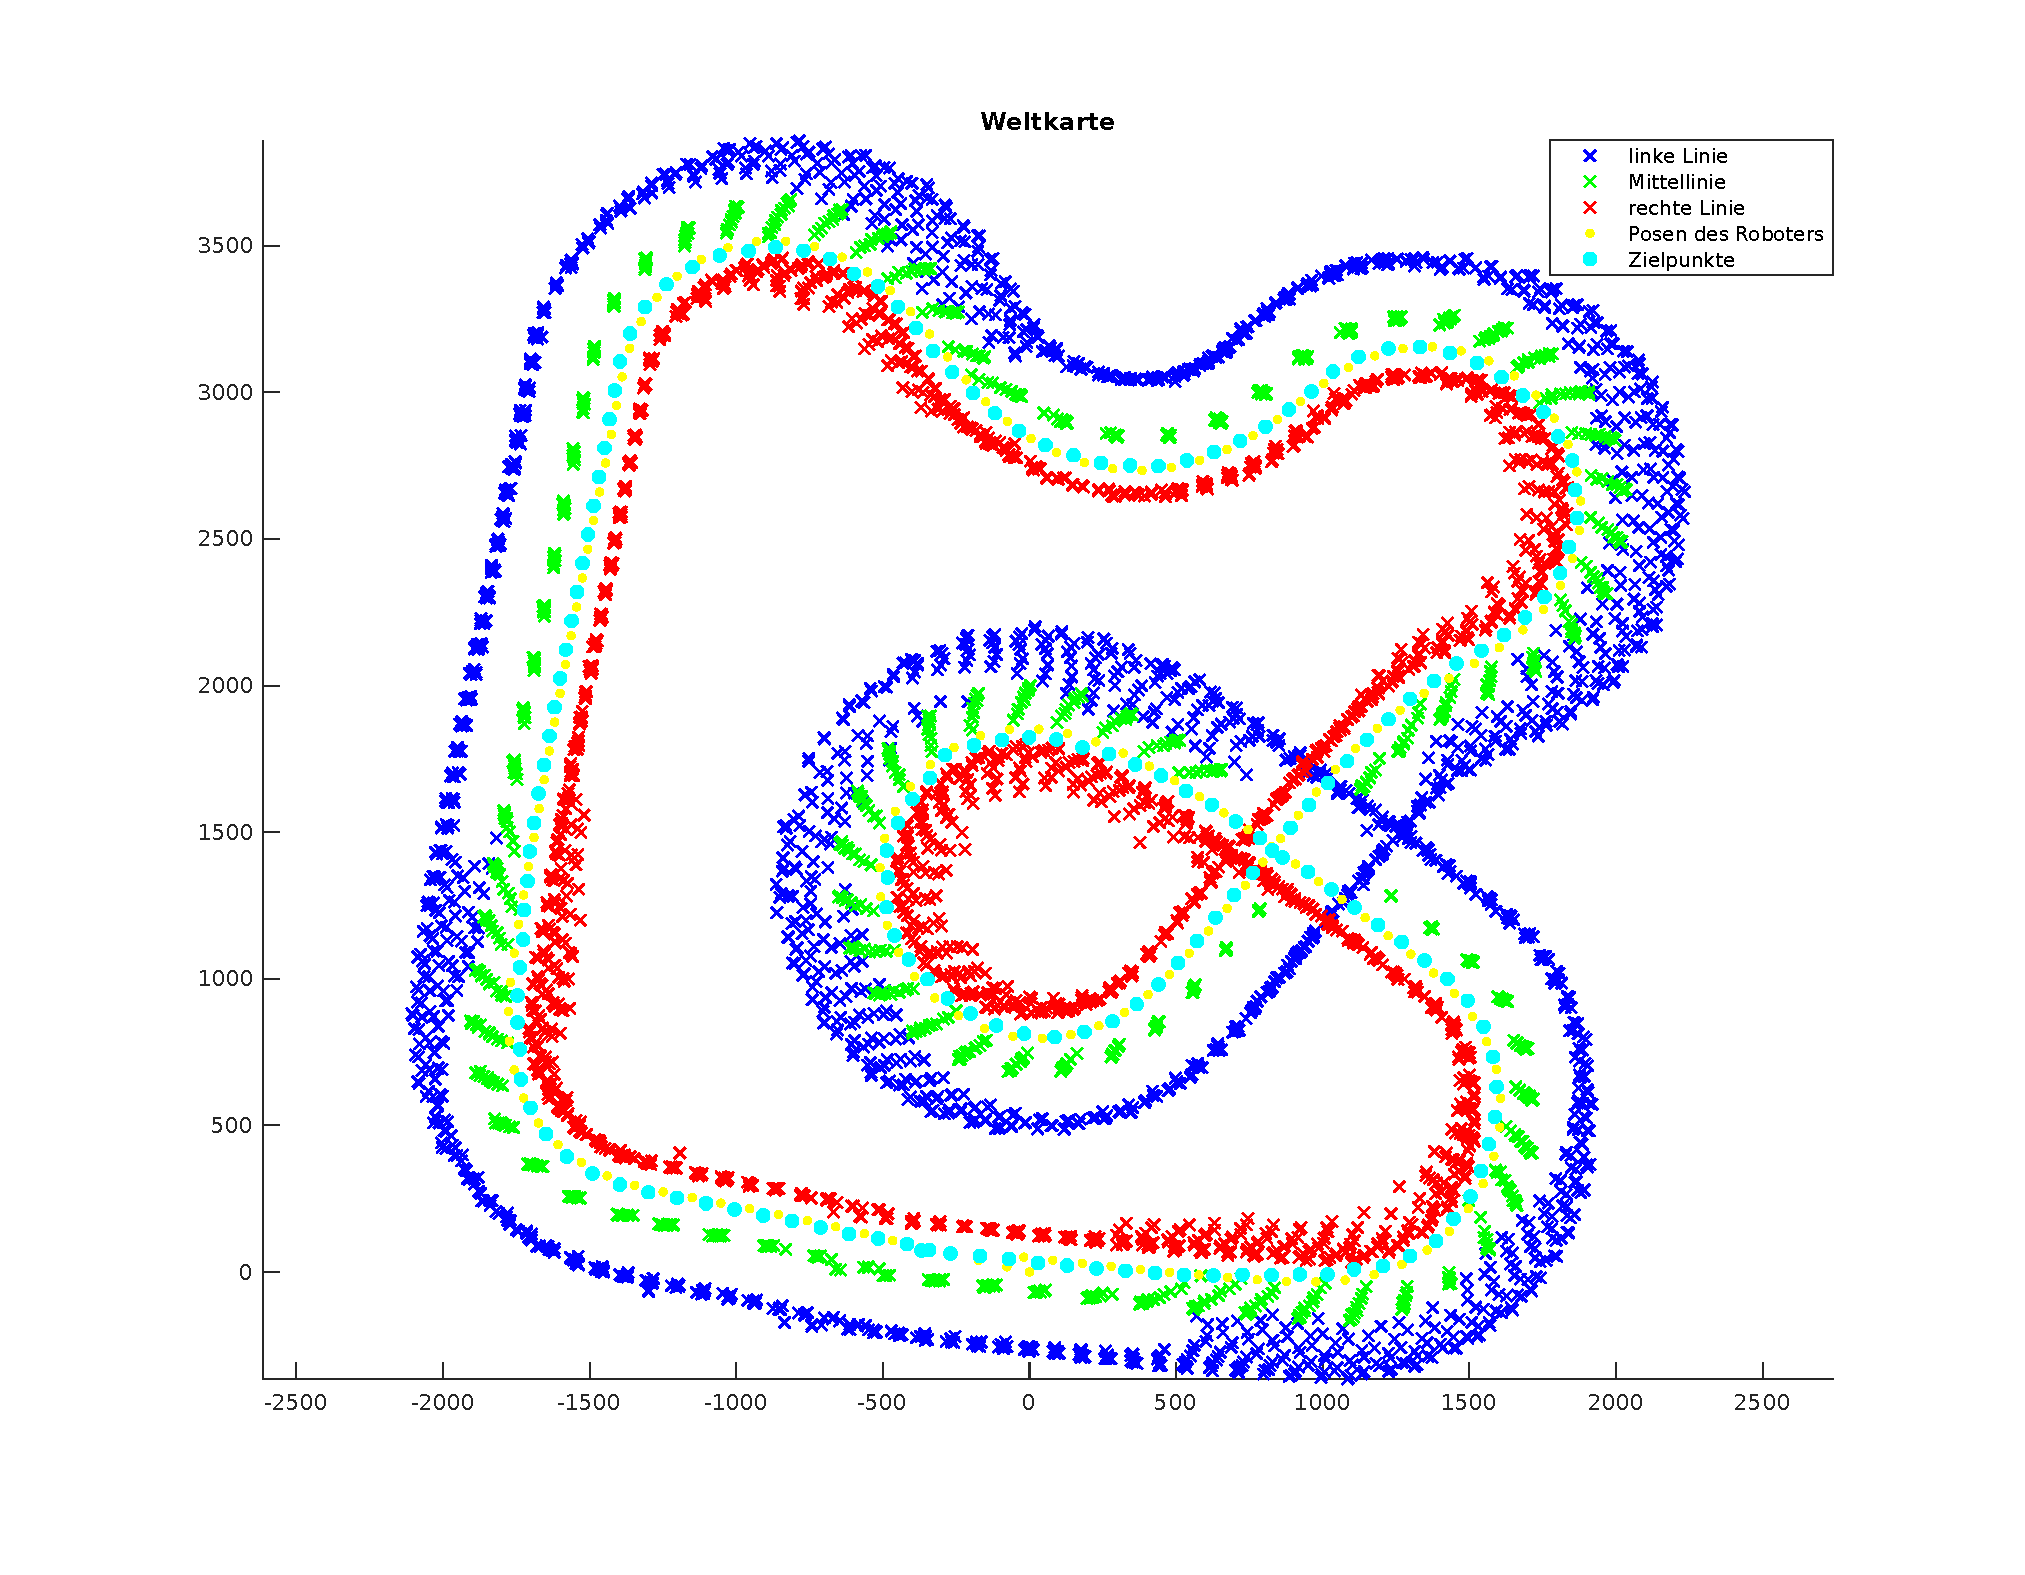
\includegraphics[height=0.31\textheight]{Weltkarte_schoen_andere_Richtung.pdf}}	
%	\includegraphics[width=0.8\textwidth]{strassenszenario_kombi_weltkarte.pdf}
	\caption{Darstellungen aufgenommener Kartendaten der Teststrecke zur Qualitätsuntersuchung}
	
\end{figure} 

Durch die Kennzeichnung von rechter und linker Randlinie ist die Fahrtrichtung zu erkennen. In der Rechtskurve fällt auf, dass eine zu starke Krümmung der Linien erkannt wurde. Die Ursache dieses Fehlers liegt in der noch leider insuffizienten Bildentzerrung. Dies führt dazu, dass der Roboter die steileren Rechtskurven etwas schneidet. Nichts desto trotz gelingt die Fahrt auf dem Parcours auch in entgegengesetzter Richtung, wie Abbildung~\ref{fig:evaluation:riverflow:weltkarte:andere_Richtung} zeigt.